\chapter{Technical Development}
\setcounter{section}{0}

This chapter describes the research and engineering foundations of this FDP: how the recognition
solution is structured into independent stages, the methodological investigations that informed the
choice of algorithms and hyperparameters, and the functional capabilities provided by each stage.
It also details the execution environment and the requirements that drove the architectural design.
Finally, it describes the experimental datasets that feed the recognition pipeline.

\section{Solution design}
\label{sec:system_design}

The solution is structured as a modular three-stage architecture, integrating research-driven
methods across data preparation, model training and evaluation, and runtime inference. The stages
are physically separated (different processes and different machines in the execution environment)
but share a single source of truth for data formats and trained model artefacts, so a checkpoint
produced during model training can be served unchanged during runtime inference.
Figure~\ref{fig:system_overview} shows the solution architecture and its execution flow.

\clearpage
\begin{landscape}
    \thispagestyle{empty}
    \begin{figure}[H]
        \centering
        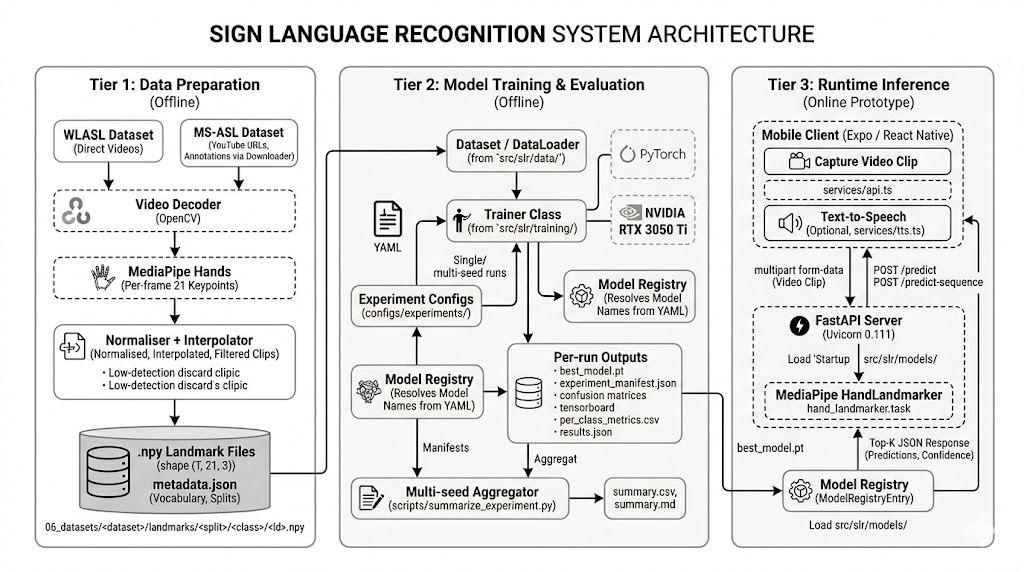
\includegraphics[width=\linewidth,height=1.0\textheight,keepaspectratio]{./images/architecture/system_overview.png}
        \caption{Solution architecture showing the data preparation, training and evaluation, and runtime inference stages. Source: self-created from the implemented pipeline.}
        \label{fig:system_overview}
    \end{figure}
\end{landscape}
\clearpage

\subsection{Stage 1: Data preparation}
\label{subsec:data_preparation}

The data preparation stage converts raw benchmark videos into landmark sequences that can be used
by the training and inference stages. It corresponds to the first two stages of the recognition
pipeline introduced in Section~\ref{subsec:recognition_pipeline}, namely video acquisition and
decoding, and landmark extraction and normalisation. This section decomposes those stages into five
execution phases:

\begin{enumerate}
    \item \textbf{Video acquisition.} The input is the official Word-Level American Sign Language
          (WLASL) distribution or the Microsoft American Sign Language (MS-ASL) annotation files.
          WLASL clips are downloaded from the dataset distribution, while MS-ASL clips are
          reconstructed from the referenced YouTube videos. The output is a local set of labelled
          video clips aligned with their gloss and split metadata.
    \item \textbf{Clip decoding and temporal trimming.} OpenCV decodes each video frame by frame.
          For MS-ASL, each source video is trimmed with the per-instance \texttt{(start\_time,
              end\_time)} pair. The output is an ordered frame sequence for one sign instance.
    \item \textbf{Hand landmark extraction.} MediaPipe Hands estimates 21 three-dimensional
          landmarks per valid frame. The output for each frame is a structured hand representation
          with coordinates for the wrist, finger joints and fingertips.
    \item \textbf{Geometric normalisation and missing-frame handling.} Each frame is wrist-centred
          and length-normalised by the wrist-to-middle-finger distance. Frames where MediaPipe fails
          to detect a hand are linearly interpolated from neighbouring valid frames, and clips whose
          detection rate falls below 0.3 are discarded.
    \item \textbf{Serialisation.} Each surviving clip is stored as a per-clip \texttt{.npy} array
          of shape $(T, 21, 3)$. The accompanying \texttt{metadata.json} records the dataset name,
          gloss vocabulary, split assignments and source-video identifiers.
\end{enumerate}

This stage is implemented in \texttt{src/slr/data/} and exposed through the
\texttt{scripts/extract\_landmarks\_*.py} entry points.

\subsection{Stage 2: Model training and evaluation}
\label{subsec:model_training_evaluation}

The training and evaluation stage turns landmark sequences into reproducible model comparisons. Its
execution follows four phases:

\begin{enumerate}
    \item \textbf{Configuration resolution.} The input is a YAML configuration under
          \texttt{configs/}. The file specifies the dataset path, model identifier, optimiser,
          sequence length and evaluation settings. Shared defaults are declared in
          \texttt{configs/base/gru\_attention.yaml}, and experiment-specific files override only
          the fields that change.
    \item \textbf{Model construction.} The registry in \texttt{src/slr/models/} resolves the model
          identifier into one of the implemented sequence architectures. The supported identifiers
          are \texttt{gru\_baseline}, \texttt{gru\_attention} and \texttt{transformer}.
    \item \textbf{Optimisation and evaluation.} The trainer in \texttt{training/trainer.py}
          optimises the selected architecture and evaluates it through the shared evaluator in
          \texttt{evaluation/}. The same trainer supports the multi-seed protocol used to report
          mean and standard deviation in the experiments chapter.
    \item \textbf{Artefact generation.} Each run produces a self-contained directory with the best
          checkpoint by validation Top-1, the training history, confusion matrices, per-class
          metrics and an \texttt{experiment\_manifest.json} recording git commit, hardware,
          runtime, hyperparameters and final metrics.
\end{enumerate}

The experiment-tracking code is implemented in \texttt{tracking/manifest.py} and
\texttt{tracking/git\_utils.py}.

\subsection{Stage 3: Runtime inference}
\label{subsec:runtime_inference}

The runtime inference stage integrates the trained recogniser into a mobile/server proof of
concept. Its execution follows five phases:

\begin{enumerate}
    \item \textbf{Video capture.} The React Native and Expo client in
          \texttt{03\_app/signtotext-expo/} records a short video clip with the device camera.
    \item \textbf{Request submission.} The client sends the clip to the FastAPI server in
          \texttt{04\_server/main.py} through the REST client implemented in
          \texttt{services/api.ts}.
    \item \textbf{Server-side preprocessing.} The server applies the same MediaPipe landmark
          extraction, normalisation and sequence preparation used in the data preparation stage.
    \item \textbf{Prediction.} The server loads the requested checkpoint from the model registry
          and returns Top-K predictions with confidence scores through \texttt{POST /predict}.
          The \texttt{POST /predict-sequence} endpoint provides a heuristic continuous-sequence
          variant.
    \item \textbf{Client response.} The client displays the prediction shortlist and can pass the
          Top-1 label to the text-to-speech service in \texttt{services/tts.ts}.
\end{enumerate}

The server reuses the \texttt{src/slr/} package directly, so the inference code path remains
aligned with the evaluation code path.

\subsection{Description of functional features}
\label{sec:functional_features}

The solution exposes six high-level capabilities. Each one is justified by the technical decision
it embodies, so this list doubles as a record of why the architecture took its current shape.

\begin{itemize}
    \item \textbf{F1: Landmark-based input pipeline.} Each frame is reduced from a $224 \times 224$ RGB tensor to 63 floating-point landmark coordinates, a roughly 2{,}389$\times$ dimensionality reduction. The choice removes background and skin-tone signal at source, which both shrinks the model and disconnects recognition accuracy from appearance bias.
    \item \textbf{F2: Multi-seed training protocol.} The trainer supports running the same configuration across multiple random seeds and aggregating the metrics with mean and standard deviation. Without this protocol, a single-seed Top-1 figure on a small test set is indistinguishable from noise; with it, a 2--3 percentage-point standard deviation can be reported alongside every headline number.
    \item \textbf{F3: Architecture-agnostic training loop.} The same \texttt{Trainer} accepts three model identifiers through a registry lookup: \texttt{gru\_baseline} is a bidirectional GRU architecture without attention, \texttt{gru\_attention} is the selected GRU architecture with a temporal attention layer, and \texttt{transformer} is a self-attention architecture used as a comparison baseline. This makes the architecture comparison reproducible: only the model field of the YAML changes between runs, every other variable stays fixed.
    \item \textbf{F4: Cross-dataset validation.} The same pipeline runs unmodified on WLASL and on MS-ASL. Only the dataset path and the gloss vocabulary differ between the two configurations; nothing in the model, optimiser or loss is dataset-specific, which is what makes the cross-dataset comparison fair.
    \item \textbf{F5: Reproducible experiment tracking.} Every run writes an \texttt{experiment\_manifest.json} that captures git commit, dataset metadata, hyperparameters, hardware, runtime, and final metrics in one place. A future user can reconstruct the exact configuration of any historical run from this single file.
    \item \textbf{F6: Top-K predictions in inference.} The runtime API returns Top-1 and Top-5 candidates with confidence scores instead of forcing a single answer. This matches the way the model itself is evaluated and lets the client surface a shortlist when the Top-1 confidence is low.
\end{itemize}

For example, the \texttt{experiment\_manifest.json} generated for the MS-ASL50 seed 2026 run
records the dataset identifier, random seed, split sizes, GRU+Attention configuration, hardware,
runtime, checkpoint path and final metrics, including 71.19\% Top-1 and 91.53\% Top-5 accuracy.
This is the concrete output produced by the reproducible experiment-tracking feature.

\subsection{Operational Environment}
\label{sec:operational_environment}

Training and landmark extraction were performed in the local development environment; the runtime
prototype was tested with a paired mobile client and an HTTP server.
Table~\ref{tab:operational_environment} summarises the hardware, software runtime and storage
formats under which the results in this FDP were produced.

\begin{table}[H]
    \centering
    \small
    \renewcommand{\arraystretch}{1.25}
    \caption{Operational environment for training, landmark extraction, and runtime inference.}
    \label{tab:operational_environment}
    \begin{tabular}{@{}p{4.2cm} p{9.0cm}@{}}
        \toprule
        \textbf{Environment area} & \textbf{Specification}                                                          \\
        \midrule
        Operating system          & Ubuntu 24.04 LTS (training and server); cross-platform (mobile client).         \\
        CPU                       & Multi-core x86\_64 (local laptop).                                              \\
        GPU                       & NVIDIA RTX 3050 Ti Laptop, 4\,GB VRAM, CUDA 12.x.                               \\
        Python                    & 3.10 (project); 3.11 supported via \texttt{requires-python = ">=3.10"}.         \\
        Deep learning framework   & PyTorch 2.x with CUDA support.                                                  \\
        Pose estimation           & MediaPipe Hands 0.10+ (\texttt{HandLandmarker}).                                \\
        Video processing          & OpenCV 4.8+.                                                                    \\
        Mobile client framework   & React Native + Expo.                                                            \\
        Backend                   & FastAPI 0.111 with Uvicorn 0.29.                                                \\
        Persistence               & JSON manifests, \texttt{.npy} landmark files, \texttt{.pt} PyTorch checkpoints. \\
        Version control           & Git.                                                                            \\
        \bottomrule
    \end{tabular}
\end{table}

The detailed installation and execution procedure is not repeated in this section. It belongs to
the user manual appendix, where the environment setup, dataset preparation, training commands,
evaluation commands and server execution procedure are described together.

\section{Requirements}
\label{sec:requirements}

\subsection{Description of requirement attributes}

For the textual description of the different identified requirements, a set of attributes has been
selected to describe each requirement. Below is a description of the meaning of each attribute
used:

\begin{itemize}
    \item \textbf{Code}: A unique abbreviated identifier for the requirement. It is constructed using the requirement type code followed by a hyphen and three digits. Requirements are divided into functional and non-functional requirements. The codes used are \textbf{FR} for Functional Requirements and \textbf{NFR} for Non-Functional Requirements. For example: \texttt{FR-001}.

    \item \textbf{Name}: Extended identification of the requirement.

    \item \textbf{Description}: A basic description of the identified requirement.

    \item \textbf{Source}: Indicates the source through which the requirement was identified. This value usually corresponds to one or more use case codes.

    \item \textbf{Necessity}: Determines the degree of implementation required for the requirement. The possible values are:
          \begin{itemize}
              \item \textbf{Essential}: The requirement must be implemented.
              \item \textbf{Desirable}: It is preferable to implement the requirement, but it is not mandatory.
              \item \textbf{Optional}: The requirement may be implemented, but it is neither important nor mandatory.
          \end{itemize}

    \item \textbf{Priority}: Defines the importance of the requirement, allowing the order in which requirements are included in the design and implementation process to be established. The possible values are:
          \begin{itemize}
              \item \textbf{High}: The requirement must be implemented in the early stages of development.
              \item \textbf{Medium}: The requirement should be implemented once high-priority requirements have been completed.
              \item \textbf{Low}: The requirement should be implemented in the final stages of development. These requirements do not affect the correct functioning of the system.
          \end{itemize}

    \item \textbf{Stability}: Defines the stability of the requirement throughout the software life cycle. This indicates whether the requirement may be modified during the life cycle. The possible values are:
          \begin{itemize}
              \item \textbf{Stable}: The requirement will not change during the system life cycle.
              \item \textbf{Unstable}: The requirement may change during the system life cycle.
          \end{itemize}

    \item \textbf{Verifiability}: Defines the degree to which a requirement can be verified, that is, the extent to which it is possible to confirm that the requirement has been implemented in the developed system. The possible values are:
          \begin{itemize}
              \item \textbf{High}: It is possible to verify that the requirement has been implemented. These requirements usually correspond to core system functionalities.
              \item \textbf{Medium}: It is possible to verify that the requirement has been implemented, but it requires complex testing or inspection of the source code.
              \item \textbf{Low}: It is difficult, or in some cases impossible, to verify whether the requirement has been implemented.
          \end{itemize}
\end{itemize}

\subsection{Functional Requirements}
\label{sec:functional_requirements}

The system specifies four functional requirements covering the core recognition pipeline (FR-001,
FR-002), the experiment-tracking infrastructure (FR-003), and statistical validation through
multi-seed training (FR-004).

\requirement{./tables/requirement_FR_001}{FR-001: Landmark extraction from video clips}{tab:requirement_FR_001}
\requirement{./tables/requirement_FR_002}{FR-002: Word-level sign classification}{tab:requirement_FR_002}
\requirement{./tables/requirement_FR_003}{FR-003: Reproducible experiment tracking}{tab:requirement_FR_003}
\requirement{./tables/requirement_FR_004}{FR-004: Multi-seed training support}{tab:requirement_FR_004}
\FloatBarrier

\subsection{Non-functional Requirements}
\label{sec:non_functional_requirements}

Three non-functional requirements characterise quality attributes of the system: runtime
performance (NFR-001), code quality and modularity (NFR-002), and documentation completeness
(NFR-003).

\requirement{./tables/requirement_NFR_001}{NFR-001: Inference latency}{tab:requirement_NFR_001}
\requirement{./tables/requirement_NFR_002}{NFR-002: Modular code architecture}{tab:requirement_NFR_002}
\requirement{./tables/requirement_NFR_003}{NFR-003: Documentation completeness}{tab:requirement_NFR_003}
\FloatBarrier

% =============================================================================
\section{Datasets}
\label{sec:datasets}
% =============================================================================

This FDP spans two recognition tasks with different data requirements: hand localisation from still
images and word-level sign language recognition from video. Six datasets are therefore used across
the experimental pipeline. This section formalises the properties of each dataset by first defining
a common set of descriptive attributes, then presenting a comparative table and finally describing
each dataset with the same structure: metadata and technical specifications, composition and
volume, source, and preparation.

% 3.X.1 Attribute Definitions
\subsection{Dataset Attribute Definitions}
\label{subsec:dataset_attributes}

To ensure a consistent and unambiguous characterisation of every dataset, the following attributes
are used in Table~\ref{tab:datasets_comparison}. Each attribute captures a distinct dimension
relevant to dataset selection, reproducibility, and the interpretation of experimental results:

\begin{itemize}

    \item \textbf{ID}: A unique alphanumeric identifier assigned to each dataset within this FDP. The prefix \texttt{DS-} followed by a two-digit index allows unambiguous cross-referencing in subsequent chapters when reporting experimental configurations and results.

    \item \textbf{Name}: The official or widely-used name of the dataset as it appears in the literature or on its hosting platform.

    \item \textbf{Year}: The year of original publication or first public release. This contextualises the dataset within the chronological development of the field and helps evaluate whether it reflects current data collection practice.

    \item \textbf{Task}: The specific sub-task for which the dataset was designed. Three task categories appear in this FDP:
          \begin{itemize}
              \item \textbf{Hand Detection}: the dataset provides annotated bounding boxes or segmentation masks marking the location of hands in images.
              \item \textbf{Letter Recognition}: the dataset provides labelled static images of individual American Sign Language (ASL) letter signs.
              \item \textbf{Word Recognition}: the dataset provides labelled video clips of complete ASL word signs, requiring temporal modelling.
          \end{itemize}

    \item \textbf{Samples}: The total number of annotated data instances. For image datasets, this equals the number of images; for video datasets, it equals the number of individual video clips. Where a subset of the full dataset was used in this FDP, this is noted in the individual descriptions.

    \item \textbf{Classes}: The number of distinct output categories. For hand detection datasets this is always 1 (the single \textit{hand} class); for sign language datasets it corresponds to vocabulary size, meaning the number of distinct letters or word glosses.

    \item \textbf{Format}: The storage format and annotation type of the raw data. This attribute specifies whether instances are static images or video clips, the image resolution where relevant, and the form of ground-truth annotation, such as bounding box coordinates in XML, pixel-level segmentation masks, image class labels or video-level class labels.

    \item \textbf{Input Representation}: Whether the models trained on this dataset consume \textit{pixel-based} data (raw RGB or greyscale image/video frames) or \textit{landmark-based} data (structured three-dimensional keypoint coordinates extracted by a pose estimator such as MediaPipe). Pixel-based inputs preserve full visual detail but are high-dimensional and sensitive to background, lighting and signer appearance. Landmark-based inputs are compact and less exposed to visual variability, at the cost of depending on a reliable keypoint extractor.

\end{itemize}

% 3.X.2 Comparative Overview
\subsection{Comparative Overview}
\label{subsec:dataset_overview}

Table~\ref{tab:datasets_comparison} provides a high-level comparison of the six datasets used in
this FDP. Datasets DS-01 and DS-02 support the hand localisation pipeline. Datasets DS-03 and DS-04
were used in the initial letter-level classification phase, which was later superseded by
word-level recognition. Datasets DS-05 and DS-06 are the video benchmarks used for the final
landmark-based ASL recognition pipeline.

\begin{table}[H]
    \centering
    \scriptsize
    \setlength{\tabcolsep}{3pt}
    \renewcommand{\arraystretch}{1.25}
    \caption{Comparative overview of all datasets used in this FDP.}
    \label{tab:datasets_comparison}
    \begin{tabular}{@{}p{0.8cm} p{2.7cm} p{0.7cm} p{2.0cm} p{1.45cm} p{1.3cm} p{2.25cm}@{}}
        \toprule
        \textbf{ID} & \textbf{Name}       & \textbf{Year} & \textbf{Task}  & \textbf{Samples} & \textbf{Classes} & \textbf{Format}            \\
        \midrule
        DS-01       & EgoHands            & 2015          & Hand Detection & 4,800            & 1                & Images + seg.\ masks       \\
        DS-02       & Kaggle Hand Dataset & 2023          & Hand Detection & $\sim$4,200      & 1                & Images + BBox (XML)        \\
        DS-03       & Sign Language MNIST & 2017          & Letter Recog.  & 34,627           & 24               & 28$\times$28 greyscale CSV \\
        DS-04       & ASL Alphabet        & 2018          & Letter Recog.  & 87,000           & 29               & 200$\times$200 RGB JPG     \\
        DS-05       & WLASL               & 2020          & Word Recog.    & 21,083           & 2,000            & RGB video clips            \\
        DS-06       & MS-ASL              & 2018          & Word Recog.    & 25,513           & 1,000            & RGB video clips, YouTube   \\
        \bottomrule
    \end{tabular}
\end{table}

% 3.X.3 Hand Detection Datasets
\subsection{Hand Detection Datasets}
\label{subsec:datasets_hd}

Datasets DS-01 and DS-02 are used jointly to train the hand localisation module based on You Only
Look Once version 8 nano (YOLOv8n). Combining the two sources increases viewpoint diversity: an
egocentric-only detector may fail when the camera is positioned at eye level, while a detector
trained only on third-person images may struggle with first-person perspectives. After merging,
duplicate removal and a stratified train/validation/test split, the combined training set comprises
approximately 5,223 annotated images.

\subsubsection*{DS-01: EgoHands}

\paragraph{Metadata and technical specifications.} EgoHands, introduced by Bambach et al.~\cite{bambach2015egohands}, is an egocentric hand
localisation dataset published in 2015. Ground-truth annotations are stored as pixel-level
segmentation polygons in MATLAB \texttt{.mat} files. The input representation used in this FDP is
pixel-based.

\paragraph{Composition and volume.} The dataset contains approximately 4,800 labelled frames extracted from 48 video recordings. Most
frames contain two visible hands and include overlap or occlusion cases during everyday
interactions such as card games, chess and jigsaw puzzles.

\paragraph{Source.} Indiana University collected the videos using a GoPro camera mounted on the chest of an observer
watching another person. This first-person perspective makes the dataset useful for close-range
hand detection but limits its viewpoint diversity.

\paragraph{Preparation.} The segmentation polygons were converted to axis-aligned bounding boxes in YOLO format. EgoHands
was then merged with DS-02 to reduce the first-person bias of the training corpus.

\subsubsection*{DS-02: Kaggle Hand Dataset}

\paragraph{Metadata and technical specifications.} The Kaggle Hand Dataset is a collection of annotated hand images published on
Kaggle~\cite{kagglehands2023}. Ground-truth bounding boxes are provided in Pascal Visual Object
Classes (VOC) XML format. The input representation used in this FDP is pixel-based.

\paragraph{Composition and volume.} The dataset contains approximately 4,200 labelled images of hands in third-person perspectives. The
images include varied backgrounds, lighting conditions, skin tones and partial occlusions.

\paragraph{Source.} The dataset is distributed through the Kaggle platform and complements DS-01 by adding images that
are not captured from the camera wearer's viewpoint.

\paragraph{Preparation.} Bounding-box coordinates were normalised to the YOLO format used by the detection pipeline. The
joint corpus formed by DS-01 and DS-02 yielded a YOLOv8n model with approximately 98\% mean average
precision at 50\% overlap (mAP50) and 87\% mean Intersection over Union (Mean IoU) on the held-out
test split.

% 3.X.4 Letter Recognition Datasets
\subsection{Letter Recognition Datasets}
\label{subsec:datasets_lr}

Datasets DS-03 and DS-04 were used during the initial phase of the FDP, when the recognition target
was the static letter-level ASL alphabet. Both datasets cover 24 of the 26 ASL letters; the letters
\textit{J} and \textit{Z} are excluded in both cases because they require hand motion and cannot be
represented by a single static image. The two sources were merged and unified into a single
training corpus for letter classification experiments. Although this phase was later superseded by
the word-level recognition approach, these datasets remain relevant because they established the
viability of data-driven letter classification and informed the design of the preprocessing
pipeline. The input representation for both datasets is pixel-based.

\subsubsection*{DS-03: Sign Language MNIST}

\paragraph{Metadata and technical specifications.} Sign Language MNIST, hosted on Kaggle~\cite{signlanguagemnist}, mirrors the format of the MNIST
handwritten digit benchmark. Each sample is a $28 \times 28$ greyscale image distributed in CSV
format, with one label column and one pixel-intensity column per image position. The input
representation is pixel-based.

\paragraph{Composition and volume.} The dataset contains 27,455 training images and 7,172 test images, for a total of 34,627 samples.
Each sample represents one of 24 static ASL letters.

\paragraph{Source.} The dataset was constructed from ASL alphabet photographs that were rescaled and converted to the
MNIST-style format.

\paragraph{Preparation.} The low resolution and greyscale format made the dataset simple to load and normalise, but it also
removed fine-grained finger articulation details. For the initial letter-recognition experiments,
the dataset was restricted to the 24 classes shared with DS-04.

\subsubsection*{DS-04: ASL Alphabet}

\paragraph{Metadata and technical specifications.} ASL Alphabet, distributed on Kaggle~\cite{aslalphabet}, provides RGB images at a resolution of $200
\times 200$ pixels. The input representation is pixel-based.

\paragraph{Composition and volume.} The dataset contains approximately 87,000 images organised into 29 classes: the 24 static ASL
letters, the \textit{space} class and two non-letter classes (\textit{del}, \textit{nothing}). Each
class has 3,000 training images captured in a controlled environment.

\paragraph{Source.} The images were collected for static ASL alphabet recognition and provide a higher-resolution
complement to DS-03.

\paragraph{Preparation.} For integration with DS-03, images were converted to greyscale and resized to a common format. The
unified corpus contained approximately 79,000 training images and 7,000 test images covering the 24
shared letter classes.

% 3.X.5 Word Recognition Dataset
\subsection{Word Recognition Datasets}
\label{subsec:datasets_wr}

Datasets DS-05 and DS-06 are the primary benchmarks for word-level ASL recognition. WLASL is the
dataset on which the architecture was tuned, while MS-ASL was added later to validate the same
pipeline on an independent ASL corpus with a different signer distribution.

\subsubsection*{DS-05: WLASL}

\paragraph{Metadata and technical specifications.} The Word-Level American Sign Language (WLASL) dataset, published by Li et al.~\cite{li2020wlasl},
contains 21,083 video instances covering 2,000 ASL glosses. Each instance is a short RGB video
labelled with a single word-level gloss.

\paragraph{Composition and volume.} Each clip shows a single signer performing one complete sign, typically against a plain or
low-clutter background, with durations ranging from approximately one to four seconds. WLASL is
partitioned into progressively larger evaluation subsets: WLASL100, WLASL300, WLASL1000 and
WLASL2000.

\paragraph{Source.} Videos were collected from multiple online platforms, including YouTube channels maintained by ASL
educators, online courses and signing dictionaries. Qualified ASL experts manually verified the
sign production. A practical limitation is that WLASL relies on external video URLs, so some clips
become unavailable over time.

\paragraph{Preparation.} Raw RGB frames are not used as model input in this FDP. MediaPipe Hands
\cite{zhang2020mediapipehands} is applied to each frame to extract 21 three-dimensional hand
landmarks, yielding 63 scalar features per frame. The effective detection rate of MediaPipe on
WLASL clips is approximately 69\%; frames where no hand is detected are linearly interpolated from
adjacent detected frames, and each video is resampled to a fixed sequence length of 64 frames.

For the experiments described in this FDP, the following WLASL subsets were extracted and used:

\begin{itemize}
    \item \textbf{WLASL30}: The 30 most frequent glosses, used for initial architecture exploration and model selection. Split: 242 training / 56 validation / 34 test videos.
    \item \textbf{WLASL100}: The 100 most frequent glosses, used for K-Fold cross-validation and multi-split evaluation. Split: 741 training / 162 validation / 99 test videos.
    \item \textbf{WLASL300, WLASL1000, WLASL2000}: Larger subsets targeted for progressive scaling experiments, where the goal is to assess model accuracy and generalisation at increasing vocabulary sizes.
\end{itemize}

\subsubsection*{DS-06: MS-ASL}

\paragraph{Metadata and technical specifications.} The Microsoft American Sign Language (MS-ASL) dataset, published by Vaezi Joze and
Koller~\cite{joze2019msasl}, defines 25,513 video instances over 1,000 glosses. The original
release provides annotation JSON files rather than distributing the video clips directly.

\paragraph{Composition and volume.} The official split contains 16,054 training samples, 5,287 validation samples and 4,172 test
samples. The vocabulary is organised into four cumulative subsets (MS-ASL100, MS-ASL200, MS-ASL500
and MS-ASL1000) obtained by filtering on the integer label.

\paragraph{Source.} Each annotation references a YouTube URL, a per-instance \texttt{(start\_time, end\_time)} interval
and a normalised signer bounding box. Of the 25,513 declared instances, \textbf{16,816 were
successfully downloaded (65.9\% coverage)}, with split-level coverage of 74.0\% / 47.5\% / 58.0\%
for train, validation and test. The remaining clips were unavailable because the source videos had
been removed or made private.

\paragraph{Preparation.} A disk-level audit graded every downloaded clip by integrity and training viability. Only
\textbf{6} of the top-30 classes met the strict MS-ASL30 threshold of 30 train / 5 validation / 5
test surviving samples, while \textbf{17} met the MS-ASL50 threshold of 20 / 5 / 5 and \textbf{57}
met the MS-ASL100 threshold of 20 / 3 / 3. The chosen subset is therefore \textbf{MS-ASL50},
defined as the 50 classes with the largest training counts that satisfy the 20 / 3 / 3 threshold.
The subset was processed with the same MediaPipe pipeline used for WLASL: each frame was reduced to
21 three-dimensional hand landmarks and stored as a per-clip \texttt{.npy} array. After extraction,
the final per-split counts are \textbf{1,410 train / 306 validation / 236 test (1,952 total)}, with
31 source clips dropped because their mean detection rate fell below 0.3. The mean detection rate
across the surviving clips is \textbf{83.9\%}.
